\documentclass[9pt,aspectratio=169]{beamer}
\usepackage{tikz}
\usetheme{default}
\setbeamertemplate{navigation symbols}{}
\title{Cache invalidation: experiments and bounds}
\subtitle{Generated interaction study}
\author{Research group}
\date{}
\year=2026\month=11\day=5
\newcommand{\fuzzlayerA}[1]{\textit{#1}}
\newcommand{\fuzzlayerB}[1]{\fuzzlayerA{#1}}
\newcommand{\fuzzterm}[1]{\fuzzlayerB{#1}}
\newcommand{\fuzzpair}[2]{\fuzzterm{#1}: #2}
\newcommand{\fuzzunit}{steps}
\let\fuzzoriginalunit\fuzzunit
\newcommand{\fuzzcoefficient}{2}
\newcommand{\fuzzscale}[2][\fuzzcoefficient]{#1\,#2}
\definecolor{fuzzpaint}{RGB}{255,0,255}
\definecolor{fuzzsecond}{RGB}{18,137,67}
\tikzset{fuzzvertex/.style={draw,rounded corners=1pt,fill=blue!10,inner sep=1pt,minimum width=.35cm,minimum height=.25cm}}
\begin{document}
\section{Cache invalidation}
\begin{frame}[t,shrink=5]{Cache invalidation}{Composed dependencies}
\fuzzpair{Experiment}{Timing: 12\fuzzunit; estimate $\fuzzscale{x}+\fuzzscale[2]{y}$.}\par
{\renewcommand{\fuzzunit}{cycles}\let\fuzzterm\textrm\fuzzpair{LocalScope}{Timing: 7\fuzzunit.}\par}
\fuzzpair{RestoredScope}{Timing: 11\fuzzunit.}\par
\begin{columns}[onlytextwidth,b]
\begin{column}{0.46\textwidth}
\begin{description}
\item<1->[Stage 1] \textbf{We compare the} proposed solution with a reference computed from the complete input.  The estimate is $\sum_{i=1}^{n}x_i$.
\item<2->[Stage 2] \textit{The final diagram} records the order in which information crosses the partition.  The estimate is $\alpha+\beta$.
\item<2->[Stage 3] \begin{tabular}{lrr}Method&Cost&Error\\\hline
Fresh0&24&19\\
Local1&10&20\\
\end{tabular}
\end{description}
\par
\begin{flushright}
\begin{tabular}{lrr}Method&Cost&Error\\\hline
Local0&18&10\\
Fresh1&16&9\\
Cached2&4&5\\
\end{tabular}
\end{flushright}
\par
\begin{columns}[onlytextwidth,b]
\begin{column}{0.54\textwidth}
\[\begin{pmatrix}a&b\\c&d\end{pmatrix}\begin{pmatrix}x\\y\end{pmatrix}\]
\end{column}
\begin{column}{0.42\textwidth}
\[\begin{aligned}a+b&=c\\ d-e&=f\end{aligned}\]
\end{column}
\end{columns}
\end{column}
\begin{column}{0.50\textwidth}
\begin{columns}[onlytextwidth,t]
\begin{column}{0.54\textwidth}
\begin{enumerate}
\item<1-> \begin{itemize}
\item<1-> \textrm{We compare the} proposed solution with a reference computed from the complete input. Intermediate results carry both a numerical estimate and an explicit dependency set. The estimate is $\sum_{i=1}^{n}x_i$.
\end{itemize}
\item<2-> \[\begin{aligned}a+b&=c\\ d-e&=f\end{aligned}\]
\item<2-> \begin{itemize}
\item 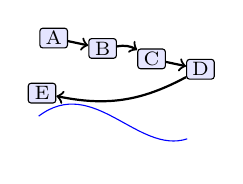
\begin{tikzpicture}[font=\scriptsize]
\begin{scope}[scale=1.1,rotate=-12]


\node[fuzzvertex] (g17n0) at (0.000,0) {A};
\node[fuzzvertex] (g17n1) at (0.577,0) {B};
\node[fuzzvertex] (g17n2) at (1.155,0) {C};
\node[fuzzvertex] (g17n3) at (1.732,0) {D};
\node[fuzzvertex] (g17n4) at (0.000,-0.65) {E};
\begin{scope}[xshift=.5pt,yshift=-.5pt]
\draw<2->[->,thick] (g17n0) -- (g17n1);
\draw<2->[->,thick] (g17n1) to[bend left=20] (g17n2);
\draw<2->[->,thick] (g17n2) -- (g17n3);
\draw<2->[->,thick] (g17n3) to[bend left=20] (g17n4);
\draw[blue] (0,-.9) .. controls (0.520,-.3) and (1.213,-1.1) .. (1.732,-.8);
\end{scope}
\end{scope}
\end{tikzpicture}
\end{itemize}
\end{enumerate}
\end{column}
\begin{column}{0.42\textwidth}
\uncover<2-3>{\begin{tabular}{lrr}Method&Cost&Error\\\hline
Fresh0&29&21\\
Global1&0&9\\
\end{tabular}}
\end{column}
\end{columns}
\end{column}
\end{columns}
\par 
\begin{tikzpicture}[font=\scriptsize]
\fill<2-3>[fuzzpaint] (0,0) rectangle (.8,.3);
\fill<3->[fuzzsecond] (1,0) rectangle (1.8,.3);
\node[anchor=west] at (2,0.15) {Witness};
\end{tikzpicture}
\only<4>{}
\end{frame}
\renewcommand{\fuzzunit}{us}
\renewcommand{\fuzzcoefficient}{2}
\renewcommand{\fuzzterm}[1]{{\textrm{#1}}}
\section{Cache invalidation}
\begin{frame}[t]{Iterative refinement}
\fuzzpair{MacroStageB}{Timing: 12\fuzzunit, retained: 9\fuzzoriginalunit.}\par
{\renewcommand{\fuzzunit}{local}\fuzzpair{FrameLocal}{Timing: 5\fuzzunit.}\par}
\fuzzpair{FrameRestored}{Timing: 8\fuzzunit; estimate $\fuzzscale{x}$.}\par
\begin{columns}[T]\begin{column}{.46\textwidth}A narrow column can change line breaking even when the underlying expression is unchanged.\end{column}\begin{column}{.46\textwidth}\begin{itemize}\item Input state\item Updated state\end{itemize}\end{column}\end{columns}
\end{frame}
\renewcommand{\fuzzunit}{steps}
\renewcommand{\fuzzcoefficient}{3}
\renewcommand{\fuzzterm}[1]{{\textrm{#1}}}
\section{Message passing}
\begin{frame}[t]{Message passing}
\fuzzpair{MacroStageC}{Timing: 12\fuzzunit, retained: 9\fuzzoriginalunit.}\par
{\renewcommand{\fuzzunit}{local}\fuzzpair{FrameLocal}{Timing: 5\fuzzunit.}\par}
\fuzzpair{FrameRestored}{Timing: 8\fuzzunit; estimate $\fuzzscale{x}$.}\par
\begin{block}{Follow-up}\fuzzterm{A revised value} depends on the preceding frame.\end{block}
\[r_{k+1}=r_k-\alpha d_k\]
\end{frame}
\end{document}
